\documentclass[cn,11pt,chinese,black]{elegantbook}
\title{Lasso优化算法的探讨和比较}
\author{组长:李宗翰,组员:蒋佩禧,袁浩然}
\cover{cover4.png}
% 本文档命令
\usepackage{array}
\newcommand{\ccr}[1]{\makecell{{\color{#1}\rule{1cm}{1cm}}}}
\usepackage{mathpazo} 
\usepackage{algorithm}  
\usepackage{algpseudocode}  
\usepackage{amsmath} 
\renewcommand{\algorithmicrequire}{\textbf{Input:}}  % Use Input in the format of Algorithm  
\renewcommand{\algorithmicensure}{\textbf{Output:}} % Use Output in the format of Algorithm  
\begin{document}  %开始写文章
	\maketitle
	\chapter*{Introduction}
	\markboth{Introduction}{Introduction}
 本文主要讨论lasso相关问题,着重介绍了近端梯度算法,在计算方面先是调用CVX程序包计算出结果,之后分别近端梯度算法(Proximal Gradient Method),加速近端梯度算法,ADMM(交替方向乘子算法)计算出结果,并对三种运算方式进行比较.
	\chapter{Lasso}
\section{引言}
 \noindent 对于线性逆问题$Y=Ax+w$,其中$A\in m×n$,$Y\in m$,且已知,w是未知噪声,那么它可以用最小二乘法求解:$\hat{x}=\operatorname{argmin}_{x}\|A x-y\|_{2}^{2}$且当m=n,且A非奇异时,解为$\hat{x}=\mathrm{A}^{-1} * y$,但是在大多数情况下,A是病态的,所以用最小二乘法求解时,微小的差别会给结果带来巨大的差异\\
为了计算这种情况下的解,1996年Robert Tibshirani提出了lasso回归,lasso回归通过构造一个l1正则化的惩罚项,使得某些系数变小,适合参数的缩减与选择,且对异常值不敏感,在解决上述问题时有着较大的优势,如下
$$\hat{x}=\operatorname{argmin}_{x}\|A x-y\|_{2}^{2}+\gamma \|\left. x\right|_{1}$$
在本文中不讨论解x ̂,而主要讨论$\min \frac{1}{2}|| A x-y||_{2}^{2}+\left.\gamma|| x\right|_{1}$,对于这个问题本文采用matlab的cvx程序包计算出结果,之后采用近端梯度算法,加速近端梯度算法,ADMM交替方向乘子算法)分别计算出结果,并比较它们之间的差异
\section{算法}
\subsection{cvx包}
\begin{lstlisting}[ language=Matlab] 
cvx_begin quiet
cvx_precision low
variable x(n)
minimize(0.5*sum_square(A*x - b) + gamma*norm(x,1))
cvx_end
\end{lstlisting}


\subsection{近端梯度算法:} 
$$x^{k+1}:=\operatorname{prox}_{\lambda^{k} \gamma\|\cdot\|_{1}}\left(x^{k}-\lambda^{k} A^{T}\left(A x^{k}-b\right)\right)$$
我们进行拆分:
$$f(x)=(1 / 2)\|A x-b\|_{2}^{2}, \quad g(x)=\gamma\|x\|_{1}$$
引入近端和梯度的运算符:
$$\nabla f(x)=A^{T}(A x-b), \quad \operatorname{prox}_{\gamma g}(x)=S_{\gamma}(x)$$
$$f(z) \approx f\left(x^{(k)}\right)+\nabla f\left(x^{(k)}\right)^{T}\left(z-x^{(k)}\right)+\frac{1}{2 \lambda}|| z-x^{(k)}||_{2}^{2}$$
$$\begin{aligned}
&x^{(k+1)}=\operatorname{argmin}_{\mathrm{z}}(f(z)+g(z))\\
&\begin{array}{l}
=\operatorname{argmin}_{z}\left(f\left(x^{(k)}\right)+\nabla f\left(x^{(k)}\right)^{T}\left(z-x^{(k)}\right)+\frac{1}{2 \lambda}|| z-x^{(k)}||_{2}^{2}+g(z)\right) \\
=\operatorname{argmin}_{z}\left(\frac{1}{2 \lambda}|| z-\left(x-\lambda \nabla f\left(x^{(k)}\right)\right)||_{2}^{2}+g(z)\right) \\
=\operatorname{prox}_{g, y}\left(x^{(k)}-\lambda \nabla f\left(x^{(k)}\right)\right) \\
=\operatorname{prox}_{g, y}\left(x^{(k)}-\lambda A^{\tau}\left(A x^{(k)}-b\right)\right)
\end{array}
\end{aligned}$$
其中前端函数prox $_{g . \gamma}(x)=S_{\gamma}(x),$ 可以由软阈值算法求出
因为 $f\left(x^{(k+1)}\right) \leq f\left(x^{(k)}\right)$, 所以求出的 $x^{(k+1)}$向最小值走了一步,依次迭代下去最
终 $f\left(x^{(k+1)}\right)-f\left(x^{(k)}\right)$ 符合精度要求时输出结果
\begin{algorithm}[h]
	\caption{Proximal gradient method}
	\label{alg::conjugateGradient}
	\begin{algorithmic}[1]
		\Require
		$x^{k}, \lambda^{k-1},$\\
		parameter $\beta \in(0,1)$ \\
		Let $\lambda:=\lambda^{k-1}$
		\Repeat
		\State  Let $z:=\operatorname{prox}_{\lambda g}\left(x^{k}-\lambda \nabla f\left(x^{k}\right)\right)$;
		\State  break if $f(z) \leq \hat{f}_{\lambda}\left(z, x^{k}\right)$;
		\State Update $\lambda:=\beta \lambda$ \\
		\Return  $\lambda^{k}:=\lambda, x^{k+1}:=z$
	\end{algorithmic}
\end{algorithm} 

\begin{lstlisting}[ language=Matlab] 
for k = 1:MAX_ITER
while 1
mal_gra = AtA*x - Atb;
z = l1(x - lam*mal_gra, lam*gamma);
if f(z) <= f(x) + mal_gra'*(z - x) + (1/(2*lam))*sum_square(z - x)
break;
end
lam = Be*lam;
end
xpr = x;
x = z;
h.opt(k) = obj(A, b, gamma, x, x);
if k > 1 && abs(h.opt(k) - h.opt(k-1)) < ABS
break;
end
end
\end{lstlisting}
\subsection{加速近端梯度算法}
在近端梯度算法的基础上,更新策略如下:
method:
$$\begin{array}{c}
y^{(k+1)}=x^{(k)}+\frac{k}{k+3}\left(x^{(k)}-x^{(k-1)}\right) \\
x^{k+1}=\operatorname{prox}_{g, y}\left(y^{(k+1)}-\lambda \nabla f\left(y^{(k+1)}\right)\right)
\end{array}$$
works for $\omega^{k}=k /(k+3)$ and similar line search as before
- faster $O\left(1 / k^{2}\right)$ convergence rate, originated with Nesterov (1983)
\begin{lstlisting}[ language=Matlab] 
 y = x + (k/(k+3))*(x - xpr);
 \end{lstlisting}
\begin{algorithm}[h]
	\caption{加速近端梯度算法}
	\label{alg::conjugateGradient}
	\begin{algorithmic}[1]
		\Require
		$y^{k}, \lambda^{k-1},$\\
		parameter $\beta \in(0,1)$ \\
		Let $\lambda:=\lambda^{k-1}$
		\Repeat
		\State  Let $z:=\operatorname{prox}_{\lambda g}\left(y^{k}-\lambda \nabla f\left(y^{k}\right)\right)$;
		\State  break if $f(z) \leq \hat{f}_{\lambda}\left(z, y^{k}\right)$;
		\State Update $\lambda:=\beta \lambda$ \\
		\Return  $\lambda^{k}:=\lambda, x^{k+1}:=z$			
	   \end{algorithmic}
\end{algorithm} 

 \begin{figure}[htb]
 	\centering
 	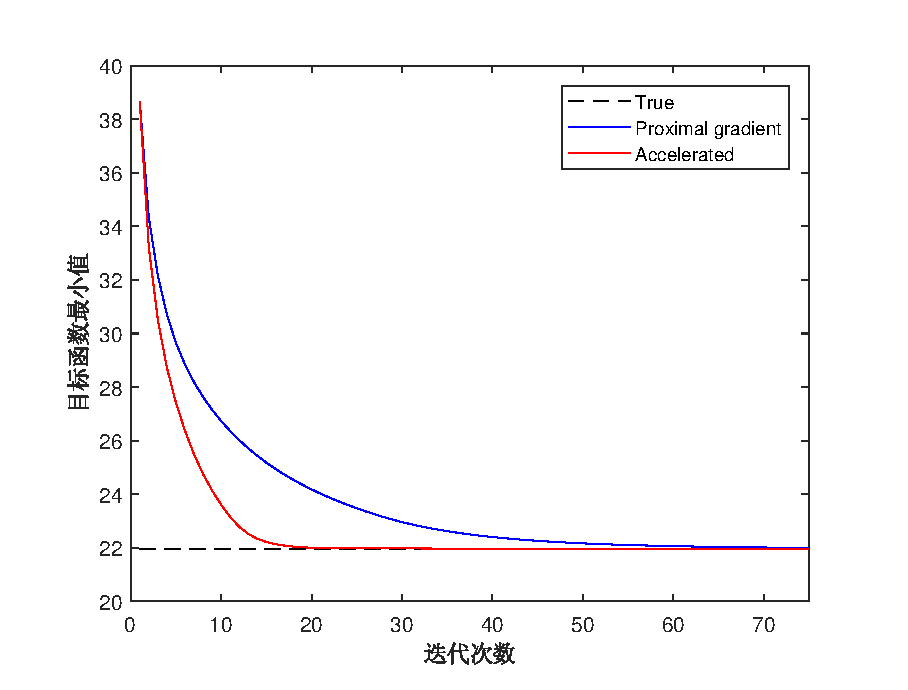
\includegraphics[width=0.6\textwidth]{1.eps}
 	\caption{近端梯度算法vs加速近端梯度算法}
 \end{figure}
\subsection{ADMM:}
$$\begin{aligned}
x^{k+1} &:=\left(I+\lambda A^{T} A\right)^{-1}\left(z^{k}-u^{k}-\lambda A^{T} b\right) \\
z^{k+1} &:=\operatorname{prox}_{\lambda \gamma\|\cdot\|_{1}}\left(x^{k+1}+u^{k}\right) \\
u^{k+1} &:=u^{k}+x^{k+1}-z^{k+1}
\end{aligned}$$





\section{数值实验}
\noindent 计算平台:IntelCore i5-8265 CPU @1.60GHz  8.00GB RAM Windows10 \\
\begin{example}
	参数设置:A=500*2500,b=A*x0+v,\\ 其中x0为n*1的稀疏矩阵,密度(在矩阵中非零元素所占的比例):0.05,v为m*1的随机生成的数组
\end{example}
 \begin{figure}[H]
	\centering
	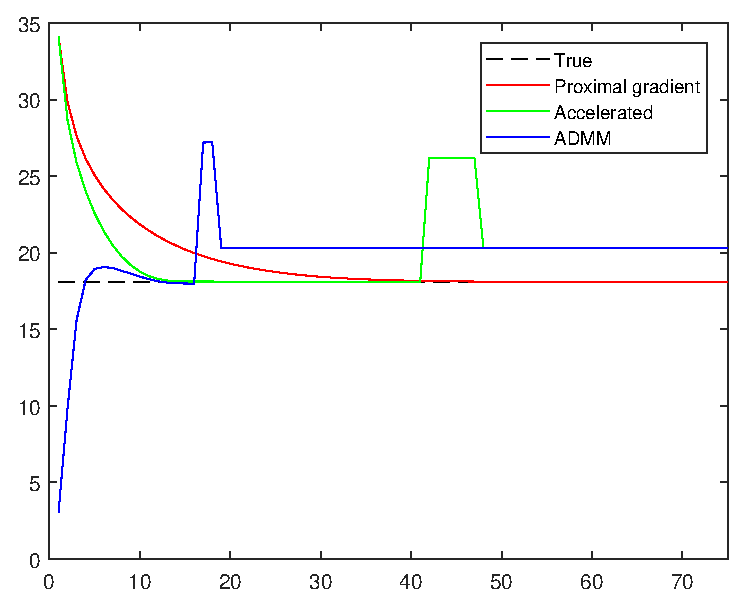
\includegraphics[width=0.6\textwidth]{lasso_comp.eps}
	\caption{Proximal gradient,Accelerated,ADMM}
\end{figure}

$$\begin{array}{llllll}
\hline \text { Method } & \text { Iterations } & \text { Time (s) } & p^{\star} & \text { Error (abs) } & \text { Error (rel) } \\
\hline \text { CVX } & 15 & 26.53 & 16.5822 & - & - \\
\text { Proximal gradient } & 127 & 0.72 & 16.5835 & 0.09 & 0.01 \\
\text { Accelerated } & 23 & 0.15 & 16.6006 & 0.26 & 1.89 \\
\text { ADMM } & 20 & 0.07 & 16.6011 & 0.18 & 1.90 \\
\hline
\end{array}$$
\begin{example}
	参数设置:A=1000*3500,b=A*x0+v,\\ 其中x0为n*1的稀疏矩阵,密度(在矩阵中非零元素所占的比例):0.05,v为m*1的随机生成的数组
\end{example}
 \begin{figure}[H]
	\centering
	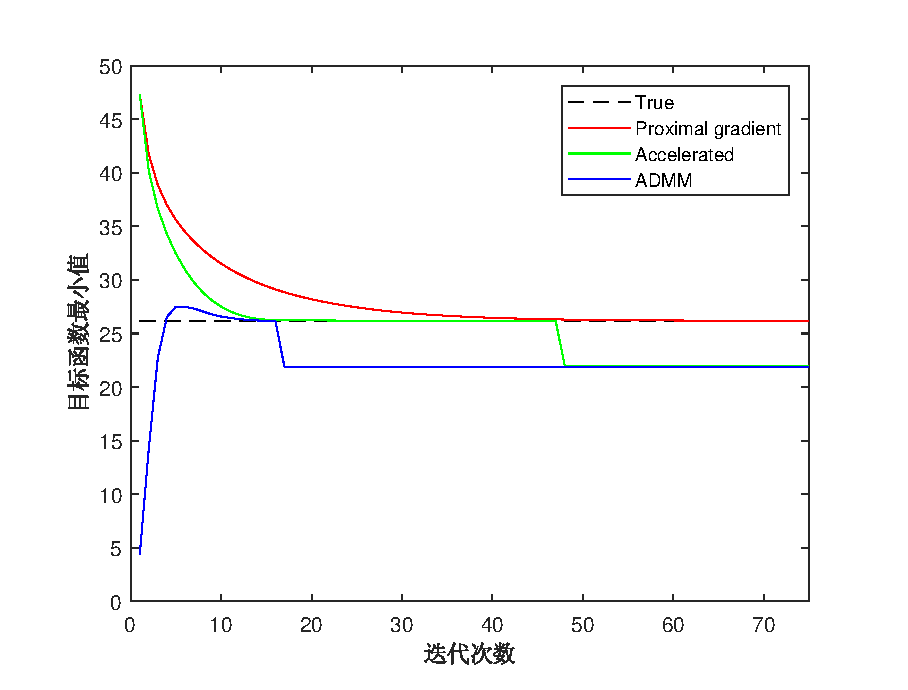
\includegraphics[width=0.6\textwidth]{2.eps}
	\caption{Proximal gradient,Accelerated,ADMM}
\end{figure}
 $$\begin{array}{llllll}
\hline \text { Method } & \text { Iterations } & \text { Time (s) } & p^{\star} & \text { Error (abs) } & \text { Error (rel) } \\
\hline \text { CVX } & 15 & 144.0169 & 23.1788 & - & - \\
\text { Proximal gradient } & 70 & 0.9906 & 23.5835 & 0.05 & 0.01 \\
\text { Accelerated } & 50 & 0.15 &  26.1053 & 3.16 & 1.54 \\
\text { ADMM } & 27 & 0.07 & 26.5721 & \3.115 & 1.53 \\
\hline
\end{array}$$
\begin{enumerate}
	在这个计算中,近端梯度算法迭代较慢,但迭代足够多的次数后,准确性较高,ADMM和加速近端梯度算法虽然迭代次数较少,但得出的低于真实目标函数的值
\end{enumerate}
\begin{example}
 参数设置:A=600*2000,b=A*x0+v,\\ 其中x0为n*1的稀疏矩阵,密度(在矩阵中非零元素所占的比例):0.05,v为m*1的随机生成的数组
\end{example}
  \begin{figure}[H]
 	\centering
 	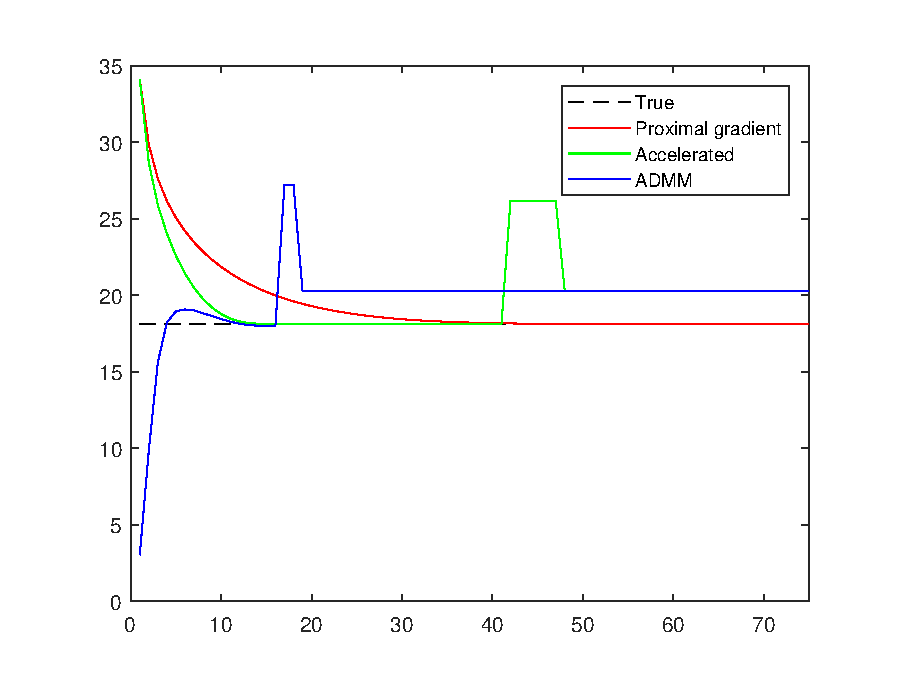
\includegraphics[width=0.6\textwidth]{3.eps}
 	\caption{Proximal gradient,Accelerated,ADMM}
 \end{figure}
 $$\begin{array}{llllll}
\hline \text { Method } & \text { Iterations } & \text { Time (s) } & p^{\star} & \text { Error (abs) } & \text { Error (rel) } \\
\hline \text { CVX } & 15 &   27.5314 & 18.5822 & - & - \\
\text { Proximal gradient } & 100 & 0.2774 & 18.5835 & 0.07 & 0.01 \\
\text { Accelerated } &59 & 0.1559 & 20.6006 & 2.26 & 1.5 \\
\text { ADMM } & 49 &  0.0589 & 20.6011 & 2.18 & 1.43 \\
\hline
\end{array}$$
\begin{enumerate}
	在这个计算中,近端梯度算法迭代较慢,但迭代足够多的次数后,准确性较高,ADMM和加速近端梯度算法虽然迭代次数较少,但得出的值高于真实目标函数的值
\end{enumerate}
\section{总结}
\noindent 本文通过三种方式计算lasso问题,并对这三种算法进行介绍,且着重介绍了近端梯度算法及其加速,我们利用数值实验计算来比较三个算法的优缺点。\\
近端梯度算法迭代较慢,但迭代足够多的次数后,准确性较高,ADMM和加速近端梯度算法虽然迭代次数较少,但显示出了较大的误差\\
将三种算法集为一体并进行比较是本文的一大优点,但是由于自身知识面所限,难免会有所错漏,有待改进。
\nocite{*} 
\bibliographystyle{plain}
\bibliography{reference.bib}
\end{document}
